\documentclass[12pt, oneside]{article}
\usepackage[letterpaper, margin=1in, headsep=0.5in]{geometry}
\usepackage[english]{babel}
\usepackage[utf8]{inputenc}
\usepackage{amsmath}
\usepackage{amsfonts}
\usepackage{amssymb}
\usepackage{tikz}
\usetikzlibrary{quotes, angles}
\usepackage{graphicx}
%\usepackage{pgfplots}
%\pgfplotsset{width=10cm,compat=1.9}
%\usepgfplotslibrary{statistics}
%\usepackage{pgfplotstable}
%\usepackage{tkz-fct}
%\usepackage{venndiagram}

\usepackage{fancyhdr}
\pagestyle{fancy}
\fancyhf{}
\rhead{\thepage \\Name: \hspace{1.5in}.\\}
\lhead{BECA / Dr. Huson / Geometry 10th Grade\\* Unit 1: Introduction to Geometry\\5 October 2018}

\renewcommand{\headrulewidth}{0pt}

\begin{document}
\subsubsection*{Exam 1b: Angle Pairs}
  \vspace{0.5cm}
  \begin{enumerate}

  \item Complete the construction of an angle bisector including the six steps.
    \begin{enumerate}
      \item Given an angle with vertex $A$.
      \item Construct circle $A$ with arbitrary radius (i.e. the radius does not matter).
      \item Label the intersections $B$ and $C$ of the angle's rays and circle $A$.
      \item Construct circle $B$  with radius $BC$. \bigskip
      \item Construct circle $\rule{2cm}{0.15mm}$  with radius $\rule{2cm}{0.15mm}$. \bigskip
      \item Label $D$, the intersection of circle $B$ and $C$. \bigskip
      \item Draw ray $\rule{2cm}{0.15mm}$.
      \bigskip
      \item Ray $\overrightarrow {AD}$ bisects $\angle A$.
    \end{enumerate}
    \vspace{3cm}
    \begin{center}
    \begin{tikzpicture}
      \draw [<->, thick] (5,6)--(0,0)--(9,0);
      \draw [fill] (0,0) circle [radius=0.05] node[below]{$A$};
      %\draw [fill] (7,0) circle [radius=0.05] node[below]{$N$};
    \end{tikzpicture}
    \end{center}
\newpage

  \item Complete the construction of a perpendicular bisector including the six steps.
    \begin{enumerate}
      \item Given the line segment $\overline{PQ}$.
      \bigskip
      \item %Construct circle $P$ with radius $\rule{2cm}{0.15mm}$.
      \bigskip
      \item %Construct circle $\rule{2cm}{0.15mm}$  with radius $\rule{2cm}{0.15mm}$.
      \bigskip
      \item %Label the intersection $P$ of the two circles.
      \bigskip
      \item Draw the line $\rule{2cm}{0.15mm}$.
      \bigskip
      \item The line $\rule{2cm}{0.15mm}$ is the perpendicular bisector of $\overline{PQ}$.
    \end{enumerate}
    \vspace{7cm}
    \begin{center}
    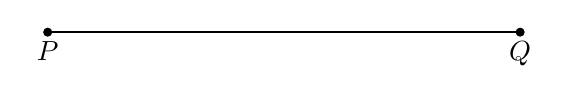
\begin{tikzpicture}
      \draw [-, thick] (0,0)--(6,0);
      \draw [fill] (0,0) circle [radius=0.05] node[below]{$P$};
      \draw [fill] (6,0) circle [radius=0.05] node[below]{$Q$};
    \end{tikzpicture}
    \end{center}
\newpage
  \item Points that are all located on the same plane are $\rule{4cm}{0.15mm}$. \bigskip

  \item Given $m \angle A=60$, $m \angle B=40$, $m \angle 1=50$, $m \angle DEF=130$, $m \angle FEG=10$. \bigskip
    \begin{enumerate}
      \item Find a pair of complementary angles. \rule{3cm}{0.15mm} \hspace{1cm} \rule{3cm}{0.15mm} \bigskip
      \item Find a pair of supplementary angles. \rule{3cm}{0.15mm} \hspace{1cm} \rule{3cm}{0.15mm} \bigskip
      \item Spicy: Find a different pair of supplementary angles. \rule{2cm}{0.15mm} \hspace{0.5cm} \rule{2cm}{0.15mm}
    \end{enumerate}

\item Identify three rays in the given plane.\\[0.25in]
  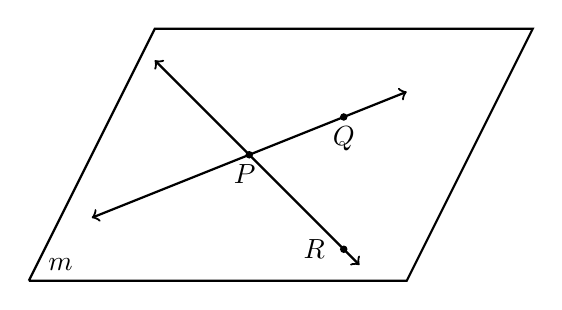
\begin{tikzpicture}[scale=0.8]
    \draw [thick](0,0) node[above right]{$\ m$} --(6,0)--(8,4)--(2,4)--(0,0);
    \draw [<->, thick] (1,1)--(6,3);
    \draw [fill] (3.5,2) circle [radius=0.05] node[below]{$P \ $};
    \draw [fill] (5,2.6) circle [radius=0.05] node[below]{$Q$};
    \draw [<->, thick] (2,3.5)--(5.25,.25);
    \draw [fill] (5,0.5) circle [radius=0.05] node[left]{$R \ $};
  \end{tikzpicture}
  \vspace{1cm}


  \item Find the value of $|\frac{2}{3}-2|-1$. \vspace{2cm}

  \item Given $\overline{ABC}$, $AC=5.8$, and $BC=1.4$.
  \begin{enumerate}
    \item Find ${AB}$.\\[1.5cm]
      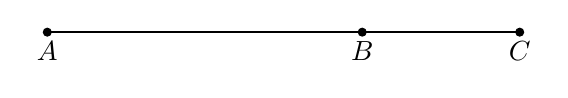
\begin{tikzpicture}
        \draw [-, thick] (1,0)--(7,0);
        \draw [fill] (1,0) circle [radius=0.05] node[below]{$A$};
        \draw [fill] (5,0) circle [radius=0.05] node[below]{$B$};
        \draw [fill] (7,0) circle [radius=0.05] node[below]{$C$};
      \end{tikzpicture} \vspace{2cm}
    \item The postulate used in this problem is the \rule{6cm}{0.15mm}.
  \end{enumerate}

\newpage
  \item Given $\overleftrightarrow{QS}$ as shown on the number line. \\[20pt] % Midpoint
    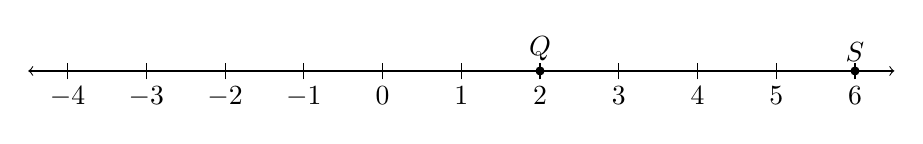
\begin{tikzpicture}
      \draw [<->] (-4.5,0)--(6.5,0);
      \foreach \x in {-4,...,6} %2 leading for diff!=1
        \draw[shift={(\x,0)},color=black] (0pt,-3pt) -- (0pt,3pt) node[below=5pt]  {$\x$};
        \draw [fill] (2,0) circle [radius=0.05] node[above] {$Q$};
        \draw [fill] (6,0) circle [radius=0.05] node[above] {$S$};
    \end{tikzpicture} \bigskip
    \begin{enumerate}
      \item Mark the point $R$, the midpoint of $\overline{QS}$.\bigskip
      \item The point $P$ is collinear with $\overleftrightarrow{QS}$ such that $Q$ is the midpoint of $\overleftrightarrow{PS}$. Mark $P$ on the line.
    \end{enumerate}\vspace{2cm}

  \item Given two perpendicular rays, $\overrightarrow{BA}$ and $\overrightarrow{BC}$, as shown. $m \angle ABD = 4x-5$, $m \angle DBC = 3x-10$. Find $m \angle DBC$.
    First label the drawing.
    \begin{flushright}
    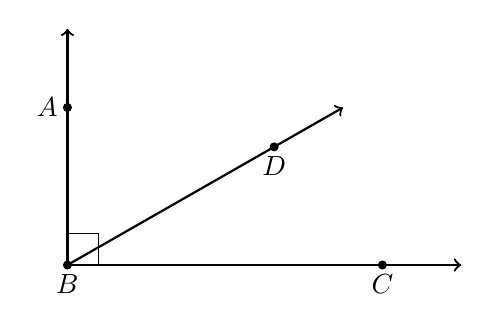
\begin{tikzpicture}[scale=1]
      \draw [<->, thick] (0,3)--(0,0)--(5,0);
      \draw [->, thick] (0,0)--(3.5, 2);
      \draw [-, thin] (0, 0.4)--(0.4, 0.4)--(0.4, 0);
      %\node at (3,.4){1};
      %\node at (6,-.6){2};
      \draw [fill] (0,0) circle [radius=0.05] node[below]{$B$};
      \draw [fill] (0,2) circle [radius=0.05] node[left]{$A$};
      \draw [fill] (4,0) circle [radius=0.05] node[below]{$C$};
      \draw [fill] (2.625, 1.5) circle [radius=0.05] node[below]{$D$};
    \end{tikzpicture}
    \end{flushright}
    %\vspace{.5cm}
    \begin{enumerate}
      \item Write a geometric equation: \rule{4cm}{0.15mm} \hspace{1cm} \rule{4cm}{0.15mm}
      \vspace{.5cm}
      \item Substitute algebraic values: \rule{4cm}{0.15mm} \bigskip
      \item Solve for $x$
      \vspace{2cm}
      %\begin{center} $x=$ \rule{1cm}{0.15mm} \end{center}
      \item Answer the question:
      \vspace{2cm}
      \item Check your answer
    \end{enumerate}

\newpage
  \item Given the situation in the diagram, answer each question. Circle True or False. \vspace{1cm}
      \begin{flushright}
      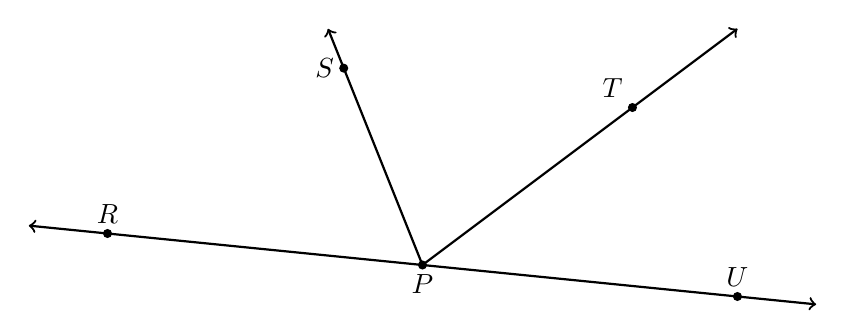
\begin{tikzpicture}[scale=1]
        \draw [->, thick] (0,0)--(4,3);
        \draw [<->, thick] (-5,.5)--(5,-.5);
        \draw [->, thick] (0,0)--(-1.2,3);
        \draw [fill] (-1,2.5) circle [radius=0.05] node[left ]{$S$};
        \draw [fill] (2.66666,2) circle [radius=0.05] node[above left ]{$T$};
        \draw [fill] (0,0) circle [radius=0.05] node[below]{$P$};
        \draw [fill] (4,-0.4) circle [radius=0.05] node[above]{$U$};
        \draw [fill] (-4,0.4) circle [radius=0.05] node[above]{$R$};
      \end{tikzpicture}
      \end{flushright}
    \begin{enumerate}
      \item True or False: $\overrightarrow{PR}$ and $\overrightarrow{UP}$ are opposite rays.\bigskip
      \item True or False: $\angle TPU$ is an obtuse angle.\bigskip
      \item True or False: $\angle RPT$ and $\angle TPU$ are supplementary angles.\bigskip
      \item True or False: $\angle RPT$ and $\angle SPT$ are adjacent. \bigskip
    \end{enumerate}


    \item 4 train to Yankee Stadium: Given $\overleftrightarrow{NYC}$, with $N=77$ and $C=161$ shown on the number line. %\\[10pt] % Midpoint
      \begin{center}
      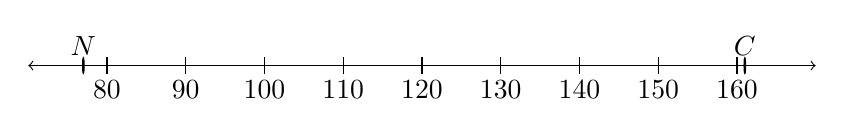
\begin{tikzpicture}[xscale=0.1]
        \draw [<->] (70,0)--(170,0);
        \foreach \x in {80,90,...,160} %2 leading for diff!=1
          \draw[shift={(\x,0)},color=black] (0pt,-3pt) -- (0pt,3pt) node[below=5pt]  {$\x$};
          \draw [fill] (77,0) circle [radius=0.1] node[above] {$N$};
          \draw [fill] (161,0) circle [radius=0.1] node[above] {$C$};
      \end{tikzpicture}
      \end{center}
      \begin{enumerate}
        \item Find the value of the midpoint $Y$, half way between 77 and 161. \vspace{4cm}
        \item Mark $Y$ on the number line in the correct location.
        \item Spicy: Find the location one-third of the distance from 86 to 161.
      \end{enumerate}

\newpage
    \item Given two vertical angles, $m \angle 1 = \frac{1}{2}(9x+11)$, $m \angle 2 = \frac{1}{2}(7x+41)$. Find $m \angle 1$.
    \begin{enumerate}
      \item First label the drawing.
      \begin{flushright}
      \begin{tikzpicture}[scale=.7]
        \draw [<->, thick] (0,-1.5)--(10,1.5);
        \draw [<->, thick] (2,3.5)--(7,-3.5);
        \node at (3,.4){1};
        \node at (6,-.6){2};
        %\draw [fill] (0,0) circle [radius=0.05] node[below]{$P$};
        %\draw [fill] (6,0) circle [radius=0.05] node[below]{$R$};
        %\draw [fill] (3,0) circle [radius=0.05] node[below]{$Q$};
      \end{tikzpicture}
      \end{flushright}
      \vspace{1cm}
      \item Write a geometric equation: \rule{4cm}{0.15mm} \hspace{1cm} \rule{4cm}{0.15mm}
      \begin{flushright} State the reason \end{flushright}
      \vspace{.7cm}
      \item Substitute algebraic values: \rule{4cm}{0.15mm}
      \item Solve for $x$
      \vspace{4cm}
      %\begin{center} $x=$ \rule{1cm}{0.15mm} \end{center}
      \item Answer the question:
      \vspace{3cm}
      \item Check your answer
    \end{enumerate}

  \end{enumerate}

\end{document}
